% Copyright 2005-2016 Airbus-EDF-IMACS-Phimeca
% Permission is granted to copy, distribute and/or modify this document
% under the terms of the GNU Free Documentation License, Version 1.2
% or any later version published by the Free Software Foundation;
% with no Invariant Sections, no Front-Cover Texts, and no Back-Cover
% Texts.  A copy of the license is included in the section entitled "GNU
% Free Documentation License".
\renewcommand{\etapemethodo}{B}
\renewcommand{\nomfichier}{docref_B222_TestKS}
\renewcommand{\titrefiche}{Kolmogorov-Smirnov goodness-of-fit test}

\Header

\MathematicalDescription{

  \underline{\textbf{Goal}} \vspace{2mm}

  This method deals with the modelling of a probability distribution of a random vector $\vect{X} = \left( X^1,\ldots,X^{n_X} \right)$. It seeks to verify the compatibility between a sample of data $\left\{ \vect{x}_1,\vect{x}_2,\ldots,\vect{x}_N \right\}$ and a candidate probability distribution previous chosen. OpenTURNS enables the use of the Kolmogorov-Smirnov Goodness-of-Fit test to answer this question in the one dimensional case $n_X =1$, and with a continuous distribution. \vspace{2mm}

  \underline{\textbf{Principle}} \vspace{2mm}

  Let us limit the case to $n_X = 1$. Thus we denote $\vect{X} = X^1 = X$. This goodness-of-fit test is based on the maximum distance between the cumulative distribution function $\widehat{F}_N$ of the sample $\left\{ x_1,x_2,\ldots,x_N \right\}$ (see \otref{docref_B11_EmpiricalCDF}{empirical cumulative distribution function}) and that of the candidate distribution, denoted $F$. This distance may be expressed as follows:
  \begin{align*}
    D = \sup_x \left|\widehat{F}_N\left(x\right) - F\left(x\right)\right|
  \end{align*}
  With a sample $\left\{ x_1,x_2,\ldots,x_N \right\}$, the distance is estimated by:
  \begin{align*}
    \widehat{D}_N = \sup_{i=1 \ldots N}\left|F\left(x_i\right)-\frac{i-1}{N} ; \frac{i}{N}-F\left(x_i\right)\right|
  \end{align*}

  The probability distribution of the distance $\widehat{D}_N$ is asymptotically known (i.e. as the size of the sample tends to infinity). If $N$ is sufficiently large, this means that for a probability $\alpha$ and a candidate distribution type, one can calculate the threshold / critical value $d_\alpha$ such that:
  \begin{itemize}
  \item if  $\widehat{D}_N>d_{\alpha}$, we reject the candidate distribution with a risk of error $\alpha$,
  \item if  $\widehat{D}_N \leq d_{\alpha}$, the candidate distribution is considered acceptable.
  \end{itemize}
  Note that $d_\alpha$ does not depend on the candidate distribution $F$ being tested, and the test is therefore relevant for any continuous distribution.

  An important notion is the so-called "$p$-value" of the test. This quantity is equal to the limit error probability $\alpha_\textrm{lim}$ under which the candidate distribution is rejected. Thus, the candidate distribution will be accepted if and only if $\alpha_\textrm{lim}$ is greater than the value $\alpha$ desired by the user. Note that the higher $\alpha_\textrm{lim} - \alpha$, the more robust the decision.

  The diagram below illustrates the principle of comparison with the empirical cumulative distribution function for an ordered sample $\left\{5,6,10,22,27\right\}$; the candidate distribution considered here is the Exponential distribution with parameters $\lambda = 0.07$, $\gamma = 0$ (see \otref{docref_B121_DistributionSelection}{standard parametric models}).

  \begin{center}
    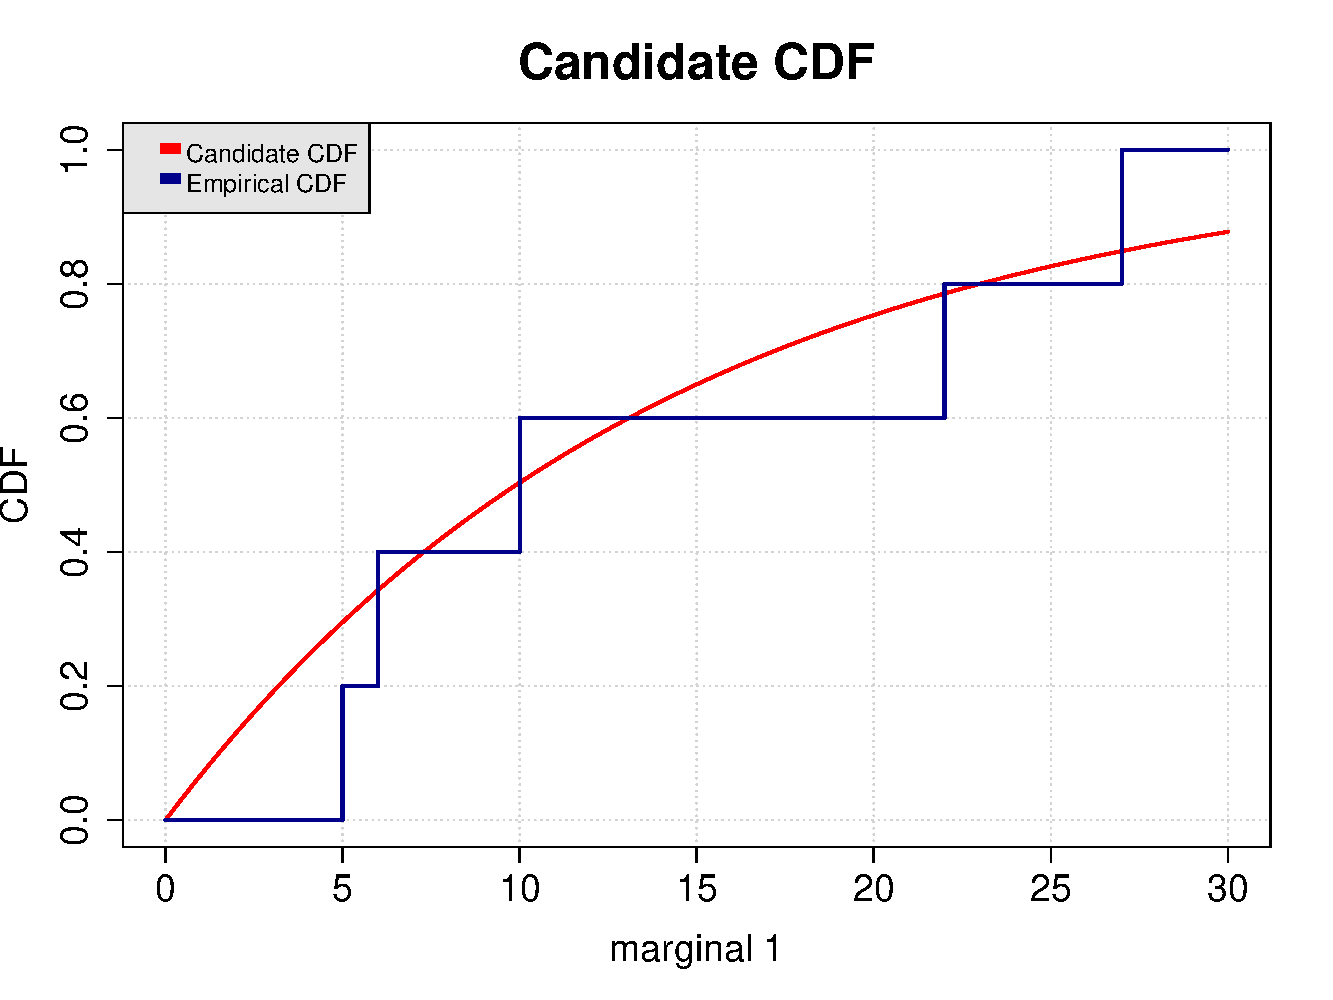
\includegraphics[scale=0.5]{Figures/kolmo.pdf}
  \end{center}
  \vspace{2mm} }
{

  This method is also referred to in the literature as Kolmogorov's Test.
}

\Methodology{
  This method is used in step B "Quantifying Sources of Uncertainty", to verify if the probability distribution is appropriate to describe the uncertainty of a component $X^i$ of the vector of unknown variables defined in step A "Specifying Criteria and the Case Study".\\

  \textbf{Input data:}\\
  $\left\{x_1,\ldots,x_N\right\}$ : data sample\\
  \textit{Distribution}: probability distribution that we are testing for goodness-of-fit \\

  \textbf{Parameters:}\\
  $\alpha$ : Level of significance for the test \\

  \textbf{Outputs:}\\
  \textit{Result}: Binary variable specifying whether the candidate distribution is rejected (0) or not (1) \\
  $\alpha_\textrm{lim}$ : $p$-value of the test
}
{
  % Références théoriques de base
  The test deals with the maximum deviation between the empirical distribtuion and the candidate distribution, it is by nature highly sensitive to presence of local deviations (a candidate distribution may be rejected even if it correctly describes the sample for almost the whole domain of variation).\\

  We remind the reader that the underlying theoretical results of the test are asymptotic. There is no rule to determine the minimum number of data values one needs to use this test; but it is often considered a reasonable approximation when $N$ is of an order of a few dozen. But whatever the value of $N$, the distance -- and similarly the $p$-value -- remains a useful tool for comparing different probability distributions to a sample. The distribution which minimizes $\widehat{D}_N$ -- or maximizes the $p$-value -- will be of interest to the analyst.

  We also point out that the calculation of $d_\alpha$ should in theory be modified if on is testing the goodness-of-fit to a parametric model where the parameters have been estimated from the same sample. The current version of OpenTURNS does not allow this modification, and the results should be therefore used with caution when the $p$-value $\alpha_\textrm{lim}$ and the desired error risk $\alpha$ are very close.

  Readers interested in Goodness of Fit tests for continuous distributions are referred to \otref{docref_B222_TestCVM}{Cramer-Von Mises test} and \otref{docref_B222_TestAD}{Anderson-Darling test} in the reference documentation.

  The following bibliographical references provide main starting points for further study of this method:
  \begin{itemize}
  \item Saporta, G. (1990). "Probabilités, Analyse de données et Statistique", Technip
  \item Dixon, W.J. \& Massey, F.J. (1983) "Introduction to statistical analysis (4th ed.)", McGraw-Hill
  \item NIST/SEMATECH e-Handbook of Statistical Methods, http://www.itl.nist.gov/div898/handbook/
  \item D'Agostino, R.B. and Stephens, M.A. (1986). "Goodness-of-Fit Techniques", Marcel Dekker, Inc., New York.
  \item Bhattacharyya, G.K., and R.A. Johnson, (1997). "Statistical Concepts and Methods", John Wiley and Sons, New York.
  \item Sprent, P., and Smeeton, N.C. (2001). "Applied Nonparametric Statistical Methods -- Third edition", Chapman \& Hall
  \end{itemize}
}
